% !TeX spellcheck = es_ES
\documentclass[12pt, titlepage]{article}
\usepackage[nottoc,notlot,notlof,numbib]{tocbibind}
\usepackage[letterpaper, margin=2.5cm]{geometry}
\usepackage[utf8]{inputenc}
\usepackage[spanish]{babel}
\usepackage{listings}
% imagenes
\usepackage{graphicx} 
\usepackage{float}
% fin imagenes
\usepackage{url}
\usepackage{color}

\definecolor{dkgreen}{rgb}{0,0.6,0}
\definecolor{gray}{rgb}{0.5,0.5,0.5}
\definecolor{mauve}{RGB}{253,151,31}
\definecolor{deepred}{RGB}{249,38,114}

\lstset{frame=tb,
	language=MATLAB,
	aboveskip=3mm,
	belowskip=3mm,
	showstringspaces=false,
	columns=flexible,
	numbers=left,
	stepnumber=1,
	basicstyle={\small\ttfamily},
	numberstyle=\tiny\color{gray},
	keywordstyle=\color{blue},
	commentstyle=\color{dkgreen},
	stringstyle=\color{mauve},
	breaklines=true,
	breakatwhitespace=true,
	tabsize=2,
	morekeywords={self, append},
	emph={},
	emphstyle=\color{deepred}
}

\title{Reporte}
\author{Barrera Pérez Carlos Tonatihu \\ Profesor: Moreno Armendariz Marco Antonio \\ Redes Neuronales \\ Grupo: 3CM2 }
\begin{document}
    \maketitle
    \tableofcontents
    \newpage
    \section{Introducción}
        Este reporte es sobre tres distintas arquitecturas de redes neuronales, las cuales son: Hamming Perceptron Simple y ADALINE. Se incluye una breve explicación sobre estas arquitecturas el como funcionan y sus diferentes representaciones para que sea fácil de entender.
        \\\\
        Además, se programaron estas tres arquitecturas, sujetas a algunas restricciones para que fuera más sencilla su elaboración, el desarrollo de estos programas fue realizado en \emph{MATLAB} ya que nos proporciona un manejo sencillo de matrices, lo cual es el principal elemento con el que trabajan estas redes neuronales. 
        \\\\
        Para verificar el correcto funcionamiento de los programas se realizaron pruebas con entradas de diferentes tamaños y valores, de igual forma se muestra en pantalla el resultado y una representación gráfica. Para complementar los resultados obtenidos se incluye un análisis de estos.
        \\\\
        Finalmente, tenemos una sección de conclusiones sobre la parte más importante de este reporte.
    \section{Marco teórico}
        \subsection{Hamming}
        Hamming es una mamada \cite{libro1}
        \subsection{Perceptron}
        \subsection{ADALINE}
    \section{Resultados experimentales}
        \subsection{Hamming}
            \begin{figure}[H]
                \begin{center}
                    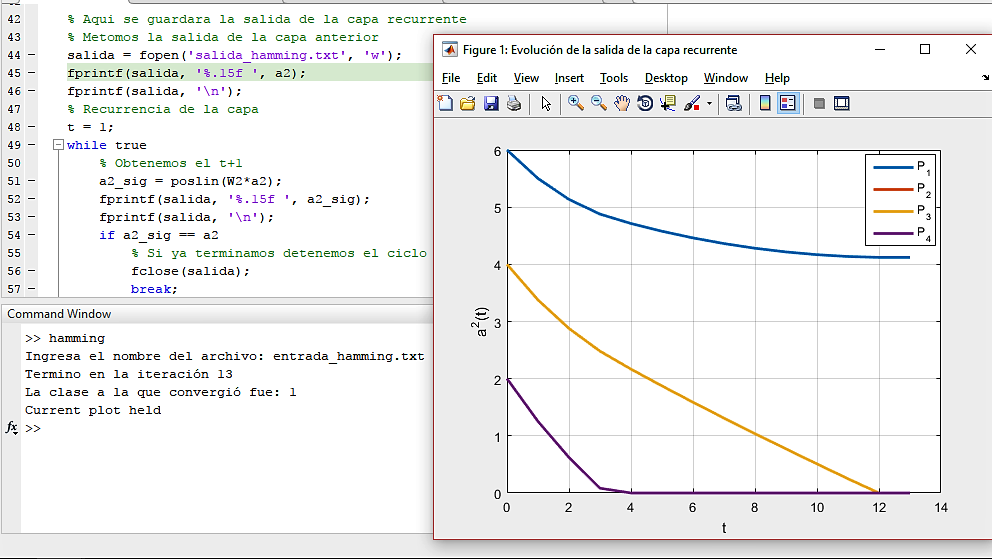
\includegraphics[width=16cm]{img/hamming1.png}
                    \caption{Prueba 1 de la red Hamming.}
                    \label{fig:hamming1}
                \end{center}
            \end{figure}
        
            \begin{figure}[H]
                \begin{center}
                    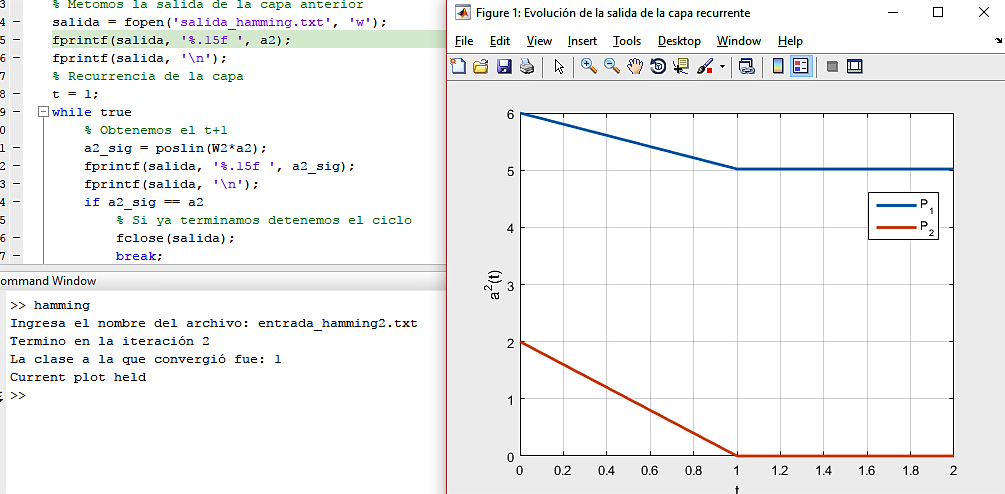
\includegraphics[width=16cm]{img/hamming2.png}
                    \caption{Prueba 2 de la red Hamming.}
                    \label{fig:hamming2}
                \end{center}
            \end{figure}
        
            \begin{figure}[H]
                \begin{center}
                    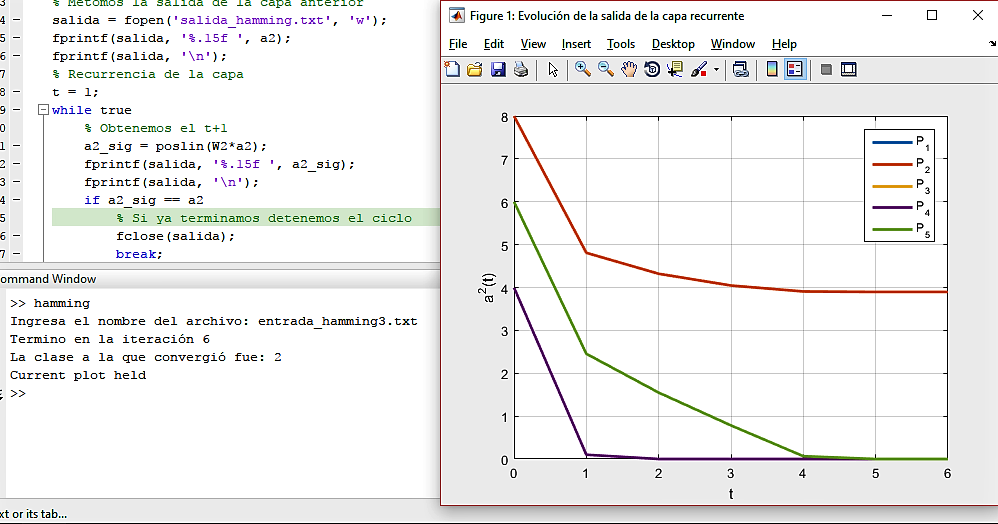
\includegraphics[width=16cm]{img/hamming3.png}
                    \caption{Prueba 3 de la red Hamming.}
                    \label{fig:hamming3}
                \end{center}
            \end{figure}
        \subsection{Perceptron}
            \subsubsection{Método Gráfico}
            \subsubsection{Aprendizaje}
        \subsection{ADALINE}
            \subsubsection{Con bias}
            Prueba 1
            \begin{figure}[H]
                \begin{center}
                    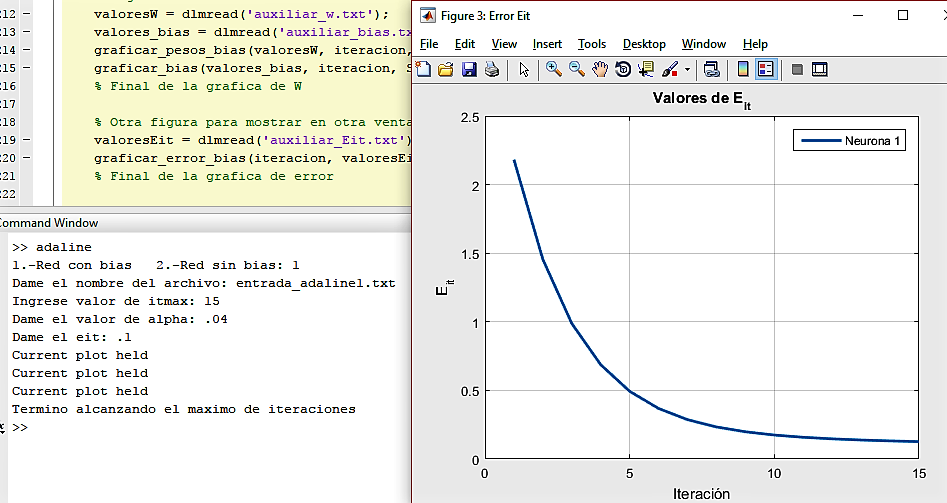
\includegraphics[width=16cm]{img/adaline1/error.png}
                    \caption{Prueba 1 de ADALINE con bias.}
                    \label{fig:adaline1error}
                \end{center}
            \end{figure}
            
            \begin{figure}[H]
                \begin{center}
                    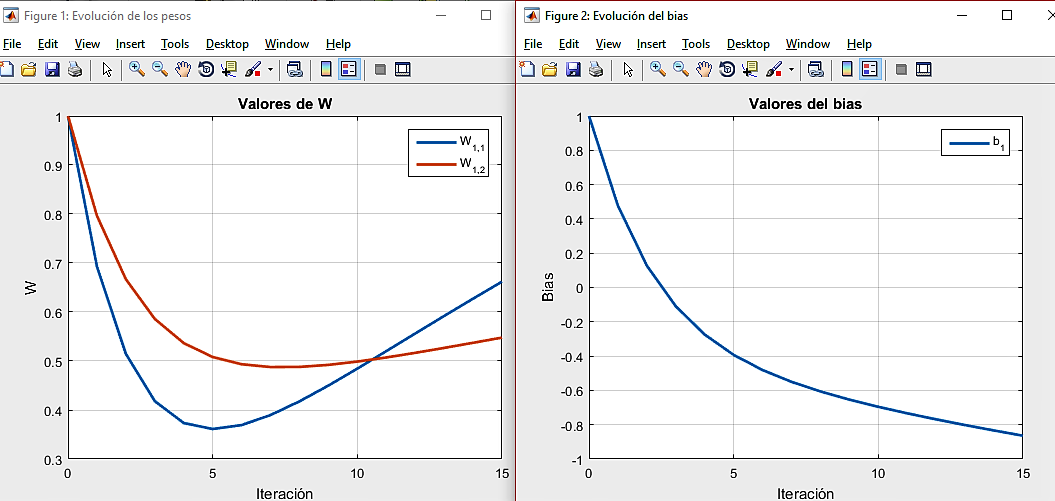
\includegraphics[width=16cm]{img/adaline1/pesosbias.png}
                    \caption{Pesos y bias en esta prueba.}
                    \label{fig:adaline1pesos}
                \end{center}
            \end{figure}
        Prueba 2
        \begin{figure}[H]
            \begin{center}
                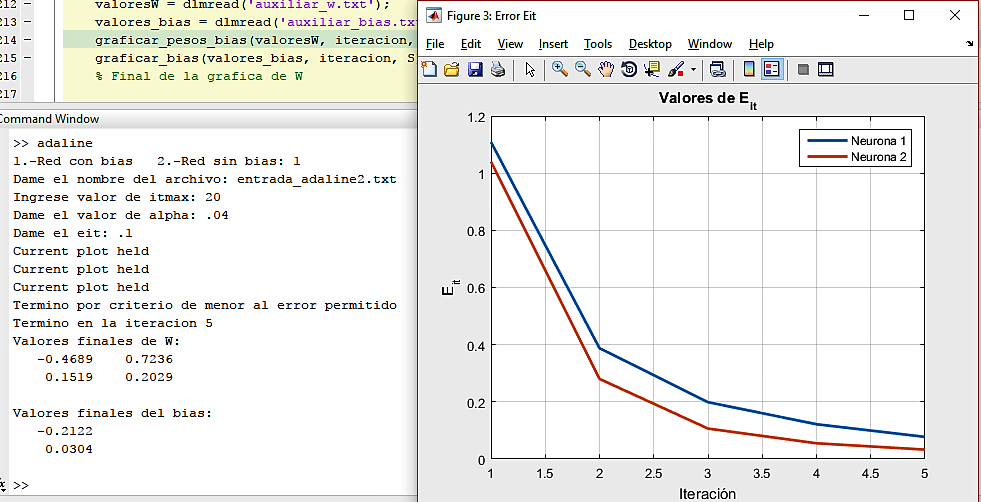
\includegraphics[width=16cm]{img/adaline2/error.png}
                \caption{Prueba 2 de ADALINE con bias.}
                \label{fig:adaline2error}
            \end{center}
        \end{figure}
        
        \begin{figure}[H]
            \begin{center}
                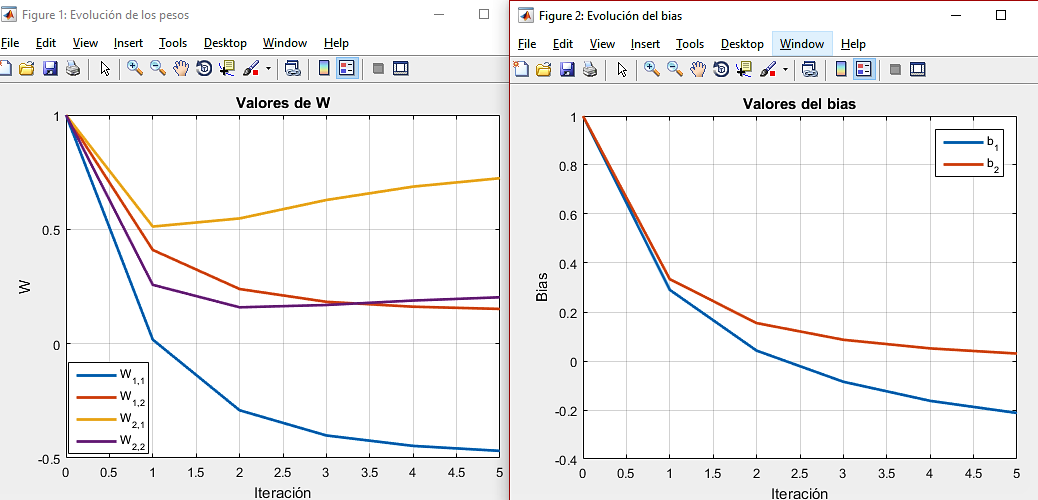
\includegraphics[width=16cm]{img/adaline2/pesosbias.png}
                \caption{Pesos y bias en esta prueba.}
                \label{fig:adaline2pesos}
            \end{center}
        \end{figure}
            \subsubsection{Sin bias}
            Prueba 1
            \begin{figure}[H]
                \begin{center}
                    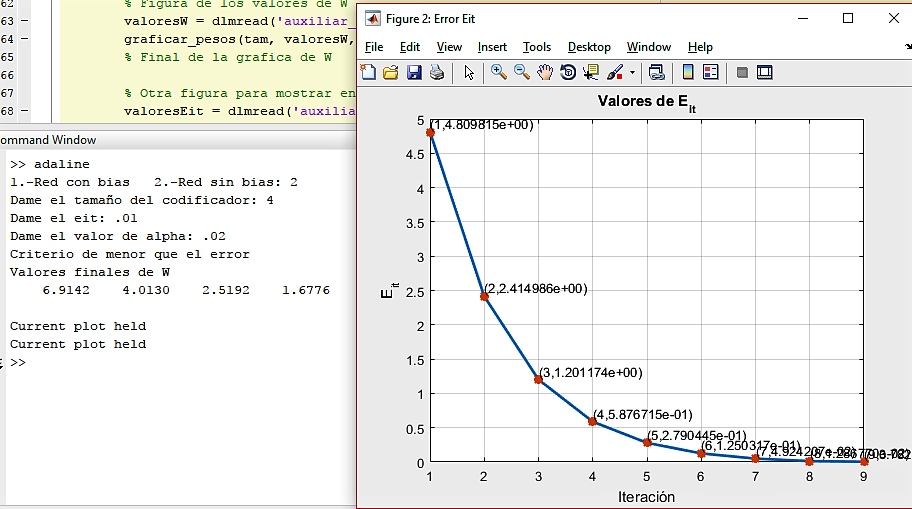
\includegraphics[width=16cm]{img/adaline3/error.png}
                    \caption{Prueba 1 de ADALINE sin bias.}
                    \label{fig:adaline3error}
                \end{center}
            \end{figure}
            
            \begin{figure}[H]
                \begin{center}
                    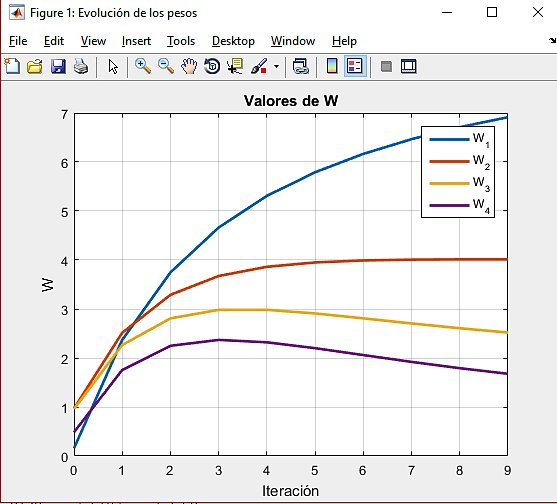
\includegraphics[width=16cm]{img/adaline3/pesosbias.png}
                    \caption{Pesos de esta prueba.}
                    \label{fig:adaline3pesos}
                \end{center}
            \end{figure}
        Prueba 2
        \begin{figure}[H]
            \begin{center}
                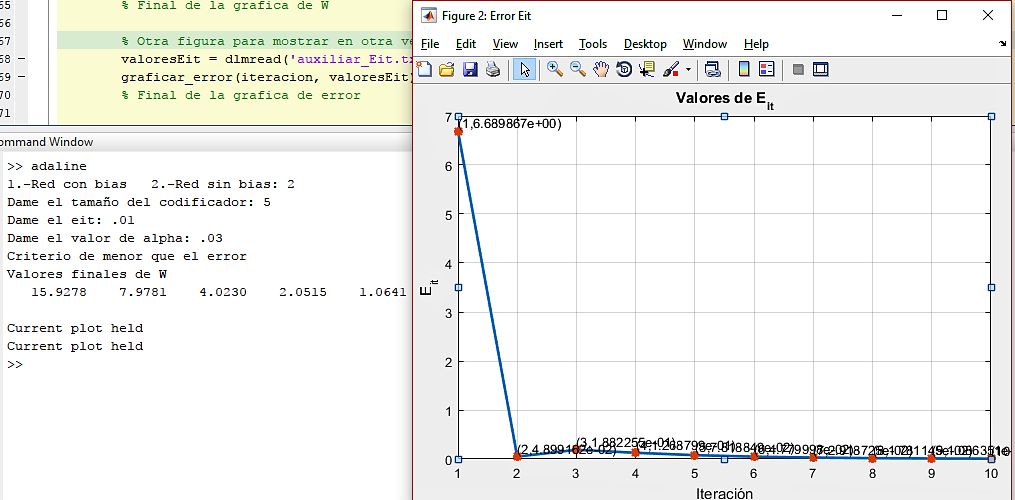
\includegraphics[width=16cm]{img/adaline4/error.png}
                \caption{Prueba 2 de ADALINE sin bias.}
                \label{fig:adaline4error}
            \end{center}
        \end{figure}
        
        \begin{figure}[H]
            \begin{center}
                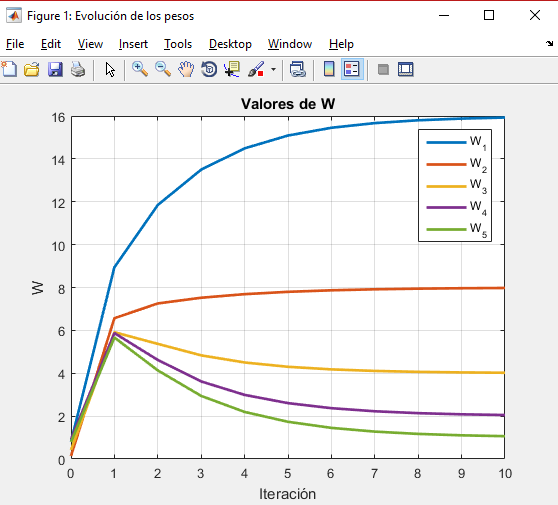
\includegraphics[width=16cm]{img/adaline4/pesosbias.png}
                \caption{Pesos de esta prueba.}
                \label{fig:adaline4pesos}
            \end{center}
        \end{figure}
    \section{Discusión de resultados}
        \subsection{Hamming}
        \subsection{Perceptron}
        \subsection{ADALINE}
    \section{Conclusiones}
    \bibliographystyle{apalike}
    \bibliography{bibliografia}
    \section{Anexo}
        En esta sección se encuentra el código de los tres programas desarrollados en MATLAB.
        \subsection{Hamming}
        \begin{lstlisting}
% Cada elemento del vector de entrada tiene solo dos posibles valores
opcion = input('Ingresa el nombre del archivo: ', 's');
archivo = dlmread(opcion);
tam = size(archivo);
% Tam de nuestros vectores prototipo
R = tam(2);

% Numero de neuronas, corresponde a cada vector prototipo
S = tam(1) - 1;

% Vector a clasificar
p = archivo(S+1, :)';

% Las filas de W1 son los vectores prototipos
% Inicializacion de W1
W1 = archivo(1:S, :);

% Cada elemento del bias es el tam del vector prototipo
% Inicializacion del bias
b1 = ones(S, 1) * R;

% Propagamos hacia adelante
a1 = purelin((W1*p)+b1);
% Fin de la capa feedforward

%Inicio de la capa recurrente
a2 = a1;
% Obtencion del valor epsilon 0 < epsilon < 1/(S-1)
epsilon = round(rand(1)*1/(S-1), 4); 
% Inicializacion y llenado de la W2 de la capa recurrente
W2 = ones(S, S);
for i = 1:S
    for j = 1:S
        if i==j
            W2(i, j) = 1;
        else
            W2(i, j) = -epsilon; 
        end;
    end;
end;

% Aqui se guardara la salida de la capa recurrente
% Metomos la salida de la capa anterior
salida = fopen('salida_hamming.txt', 'w');
fprintf(salida, '%.15f ', a2);
fprintf(salida, '\n');
% Recurrencia de la capa
t = 1;
while true
    % Obtenemos el t+1
    a2_sig = poslin(W2*a2);
    fprintf(salida, '%.15f ', a2_sig);
    fprintf(salida, '\n');
    if a2_sig == a2
        % Si ya terminamos detenemos el ciclo
        fclose(salida);
        break;
    else
        % Siguiente iteracion
        a2 = a2_sig;
    end;
    t = t + 1;
end;

% Fin de la capa recurrente
fprintf('Termino en la iteracion %d\n', t);
v = 1;
for ite = a2'
    if ite ~= 0
        break;
    else
        v = v+1;
    end;
end
fprintf('La clase a la que convergio fue: %d\n', v);
% Imprimir datos y graficar la salida de a2
a2_recurrente = dlmread('salida_hamming.txt');
figure('Name', 'Evolucion de la salida de la capa recurrente');
plot(0:t, a2_recurrente, 'LineWidth', 2);
hold;
grid;
xlabel('t');
ylabel('a^2(t)');
etiquetas = cell(1, S);
for i = 1:S
    etiquetas{i} = ['P_' num2str(i)];
end;
legend(etiquetas);
        \end{lstlisting}
        \subsection{Perceptron}
        \subsection{ADALINE}
        \begin{lstlisting}
%% Funcion principal
function adaline()
    opcion = input('1.-Red con bias   2.-Red sin bias: ', 's');
    if str2double(opcion) == 1
        adaline_bias();
    else
        % Captura de los datos
        tam = input('Dame el tam del codificador: ', 's');
        tam = str2double(tam);
        tabla_verdad = zeros(2^tam, tam+1);
        eit = input('Dame el eit: ', 's');
        eit = str2double(eit);
        alpha = input('Dame el valor de alpha: ', 's'); % 0.3
        alpha = str2double(alpha);
        N = 2^tam-1;
        W = rand(1, tam);
        auxiliar_w = fopen('auxiliar_w.txt', 'w');
        auxiliar_Eit = fopen('auxiliar_Eit.txt', 'w');
        fprintf(auxiliar_w, '%.10f ', W);
        fprintf(auxiliar_w, '\n');
        % Llenamos nuestra tabla de verdad
        for i = 0:N
            a = dec2bin(i, tam) - '0';
            tabla_verdad(i+1, 1:tam) = a;
            tabla_verdad(i+1, tam+1) = i;
        end;
        continuar = true;
        iteracion = 1;
        while continuar
            Eit = 0;
            for n = 1:N
                p = tabla_verdad(n, 1:tam)';
                a = purelin(W*p);
                t = tabla_verdad(n, tam+1);
                ed = t-a;
                Eit = Eit + ed;
                W = W + (2 * alpha * ed*p');
            end
            Eit = 1/N * Eit;
            Eit = abs(Eit);
            fprintf(auxiliar_Eit, '%.10f ', Eit);
            fprintf(auxiliar_Eit, '\n');
        
            fprintf(auxiliar_w, '%.10f ', W);
            fprintf(auxiliar_w, '\n');
            if Eit == 0
                disp('Criterio de igualdad a cero');
                break;
            elseif Eit < eit
                disp('Criterio de menor que el error');
                break;
            end
            iteracion = iteracion + 1;
        end
        fclose(auxiliar_Eit);
        fclose(auxiliar_w);
    
        % Desplegar los valores finales
        disp('Valores finales de W');
        disp(W);
        
        % Figura de los valores de W
        valoresW = dlmread('auxiliar_w.txt');
        graficar_pesos(tam, valoresW, iteracion);
        % Final de la grafica de W
        
        % Otra figura para mostrar en otra ventana
        valoresEit = dlmread('auxiliar_Eit.txt');
        graficar_error(iteracion, valoresEit)
        % Final de la grafica de error
        
        % Guardamos en un archivo
        a_final = strcat('resultado_', datestr(now, 'HH-MM_dd-mm-yyyy'));
        a_final = strcat(a_final, '.txt');
        valores_finales = fopen(a_final, 'w');
        fprintf(valores_finales, 'Valores finales de W \n');
        fprintf(valores_finales, '%.10f ', W);
        fprintf(valores_finales, '\n');
        fclose(valores_finales);
    end
end % Final de la funcion principal

%% graficar_pesos: function description
function graficar_pesos(tam, valoresW, iteracion)
    figure('Name', 'Evolucion de los pesos');
    % Grafica un vector en x y otro vector en y
    plot(0:iteracion, valoresW, 'LineWidth', 2); 
    hold;
    grid;
    % Etiquetas de los ejes
    xlabel('Iteracion');
    ylabel('W');
    
    % Titulo de nuestra grafica
    etiquetas = cell(1, tam);
    for i = 1:tam
        etiquetas{i} = ['W_' num2str(i)];
    end;
    legend(etiquetas);
    title('Valores de W');
end

%% graficar_error: function description
function graficar_error(iteracion, valoresEit)
    figure('Name', 'Error Eit');
    x = 1:iteracion;
    % Grafica un vector en x y otro vector en y
    plot(x, valoresEit, 'LineWidth', 2);
    hold;
    plot(x, valoresEit, '*', 'LineWidth', 2);
    grid;
    % Imprime las coordenadas de Eit
    strValues = strtrim(cellstr(num2str([x(:) valoresEit(:)], '(%d,%d)')));
    text(x, valoresEit, strValues, 'VerticalAlignment', 'bottom');
    % Etiquetas de los ejes
    xlabel('Iteracion');
    ylabel('E_{it}');
    % Titulo de nuestra grafica
    title('Valores de E_{it}');
end

%Con bias
function adaline_bias()
    archivo = input('Dame el nombre del archivo: ', 's');
    prueba = fopen(archivo, 'r');
    S = 0;
    targets = [];
    prototipos = [];
    R = 0;
    dimen = [];
    tipo_lectura = 0;
    while feof(prueba) == 0
        linea = fgetl(prueba);
        if linea ~= '{'
            fclose(prueba);
            datos = dlmread(archivo);
            tam = size(datos);
            S = 1;
            prototipos = datos(:, 1:tam(2)-1)';
            dimen = size(prototipos);
            targets = datos(:, tam(2))';
            R = dimen(1);
            tipo_lectura = 1;
            break;
        else
            linea = linea(2:length(linea)-1);
            proto = linea(2:find(linea==',')-2);
            tar = linea(find(linea==',')+2:length(linea)-1);
            proto = str2num(proto);
            tar = str2num(tar);
            prototipos = [prototipos proto'];
            targets = [targets tar'];
        end
    end
    if tipo_lectura == 0
        S = 2;
        dimen = size(prototipos);
        R = dimen(1);
    end   
    itmax = input('Ingrese valor de itmax: ', 's'); %5
    itmax = str2double(itmax);
    alpha = input('Dame el valor de alpha: ', 's'); % 0.3
    alpha = str2double(alpha);
    eit = input('Dame el eit: ', 's');
    eit = str2double(eit);
    W = ones(S, R);
    b = ones(S, 1);
    
    auxiliar_w = fopen('auxiliar_w.txt', 'w');
    auxiliar_bias = fopen('auxiliar_bias.txt', 'w');
    auxiliar_error = fopen('auxiliar_Eit.txt', 'w');
    fprintf(auxiliar_w, '%.10f ', W);
    fprintf(auxiliar_w, '\n');
    
    fprintf(auxiliar_bias, '%.10f ', b);
    fprintf(auxiliar_bias, '\n');
    criterio = 0;
    for iteracion = 1:itmax
        Eit = 0;
        for n = 1:dimen(2)
            p = prototipos(:, n);
            a = purelin(W*p + b);
            t = targets(:, n);
            ed = t-a;
            Eit = Eit + ed;
            W = W + (2 * alpha * ed * p');
            b = b + (2 * alpha * ed);
        end
        Eit = 1/dimen(2) * Eit;
        Eit = abs(Eit);
        fprintf(auxiliar_error, '%.10f ', Eit);
        fprintf(auxiliar_error, '\n');
        
        fprintf(auxiliar_w, '%.10f ', W);
        fprintf(auxiliar_w, '\n');
        
        fprintf(auxiliar_bias, '%.10f ', b);
        fprintf(auxiliar_bias, '\n');
        if Eit == 0
            criterio = 1;
            break;
        elseif Eit < eit
            criterio = 2;
            break;
        end
    end
    fclose(auxiliar_error);
    fclose(auxiliar_w);
    fclose(auxiliar_bias);
    
    % Figura de los valores de W
    valoresW = dlmread('auxiliar_w.txt');
    valores_bias = dlmread('auxiliar_bias.txt');
    graficar_pesos_bias(valoresW, iteracion, S, R);
    graficar_bias(valores_bias, iteracion, S);
    % Final de la grafica de W
    
    % Otra figura para mostrar en otra ventana
    valoresEit = dlmread('auxiliar_Eit.txt');
    graficar_error_bias(iteracion, valoresEit, S);
    % Final de la grafica de error
    
    if criterio == 0
        disp('Termino alcanzando el maximo de iteraciones')
    elseif criterio == 1
        disp('Termino por criterio de error igual a 0');
        fprintf('Termino en la iteracion %d\n', iteracion);
        disp('Valores finales de W:');
        disp(W);
        disp('Valores finales del bias:');
        disp(b);
    else
        disp('Termino por criterio de menor al error permitido');
        fprintf('Termino en la iteracion %d\n', iteracion);
        disp('Valores finales de W:');
        disp(W);
        disp('Valores finales del bias:');
        disp(b);
    end
    
    archivo_final = strcat('resultado_', datestr(now, 'HH-MM_dd-mm-yyyy'));
    archivo_final = strcat(archivo_final, '.txt');
    finales = fopen(archivo_final, 'w');
    fprintf(finales, 'Valores finales de W: \n');
    fprintf(finales, '%.10f ', W);
    fprintf(finales, '\n');
    
    fprintf(finales, 'Valores finales del bias: \n');
    fprintf(finales, '%.10f ', b);
    fprintf(finales, '\n');
    fclose(finales);
end


%% graficar_pesos: function description
function graficar_pesos_bias(valoresW, iteracion, S, R)
    figure('Name', 'Evolucion de los pesos');
    % Grafica un vector en x y otro vector en y
    plot(0:iteracion, valoresW, 'LineWidth', 2); 
    hold;
    grid;
    % Etiquetas de los ejes
    xlabel('Iteracion');
    ylabel('W');
    
    etiquetas = cell(1, S*R);
    k = 1;
    for i = 1:S
        for j = 1:R
            etiquetas{k} = ['W_{' num2str(i) ',' num2str(j) '}'];
            k = k+1;
        end;
    end;
    legend(etiquetas);
    title('Valores de W');
end

%% graficar_error: function description
function graficar_error_bias(iteracion, valoresEit, S)
    figure('Name', 'Error Eit');
    x = 1:iteracion;
    % Grafica un vector en x y otro vector en y
    plot(x, valoresEit, 'LineWidth', 2);
    hold;
    grid;
    % Etiquetas de los ejes
    xlabel('Iteracion');
    ylabel('E_{it}');
    % Titulo de nuestra grafica
    etiquetas = cell(1, S);
    for i = 1:S
        etiquetas{i} = ['Neurona ' num2str(i)];
    end;
    legend(etiquetas);
    % Titulo de nuestra grafica
    title('Valores de E_{it}');
end

%% graficar_bias
function graficar_bias(valores_bias, iteracion, S)
    figure('Name', 'Evolucion del bias');
    % Grafica un vector en x y otro vector en y
    plot(0:iteracion, valores_bias, 'LineWidth', 2); 
    hold;
    grid;
    % Etiquetas de los ejes
    xlabel('Iteracion');
    ylabel('Bias');
    % Titulo de nuestra grafica
    etiquetas = cell(1, S);
    for i = 1:S
        etiquetas{i} = ['b_' num2str(i)];
    end;
    legend(etiquetas);
    title('Valores del bias');
end
        \end{lstlisting}
\end{document}